\label{section:monosemantic}
In this section, we investigate individual dictionary features, highlighting several that appear to correspond to a single human-understandable explanation (i.e., that are monosemantic). We perform three analyses of our dictionary features to determine their semantic meanings: (1) \textit{Input}: We identify which tokens activate the dictionary feature and in which contexts, (2) \textit{Output}: We determine how ablating the feature changes the output logits of the model, and (3) \textit{Intermediate features}: We identify the dictionary features in previous layers that cause the analysed feature to activate.

\subsection{Input: Dictionary Features are Highly Monosemantic}
We first analyse our dictionary directions by checking what text causes them to activate. An idealised monosemantic dictionary feature will only activate on text corresponding to a single real-world feature, whereas a polysemantic dictionary feature might activate in unrelated contexts. 

% We can organize this information into a graph like Figure \ref{fig:activation_line_graph} (Left). Critically, feature activations depend not only on the token being examined, but on the preceding context.

% \begin{figure}[ht]
%     \centering
%     \begin{minipage}[b]{0.45\textwidth}
%         \centering
%         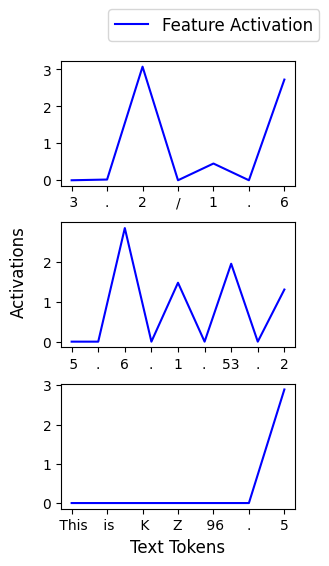
\includegraphics[width=0.9\textwidth]{images/logan/activation_line_graph.png}
%     \end{minipage}
%     % \hfill  % Optional: To make sure they are as far apart as possible.
%     \begin{minipage}[b]{0.45\textwidth}
%         \centering
%         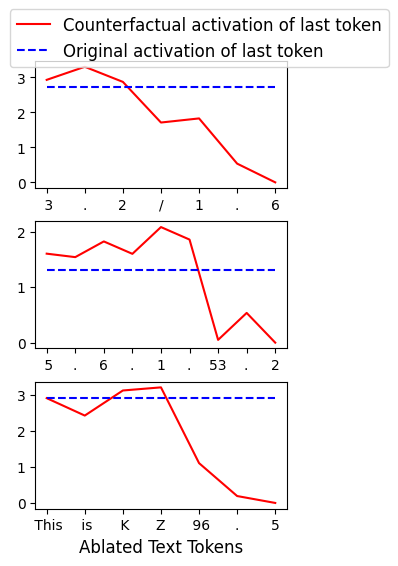
\includegraphics[width=0.9\textwidth]{images/logan/ablated_line_graph.png}
%     \end{minipage}
%     \caption{(Left) Activation of feature 756 in layer 4 in Pythia-70M, on three different token strings. This feature activates on numbers after periods. (Right) The activation of the last token in the string if the token on the x-axis is removed. For instance, in the top graph at ``/'' we would measure the activation on the final token ``6'' if the string ``3.2/1.6'' were replaced with ``3.21.6''. Note that the tokens most strongly affecting the feature activation are the final number, the period, and the number before the period.}
%     \label{fig:activation_line_graph}
% \end{figure}
 
 % To identify the most important prior tokens, we ablate each token in the sequence one at a time, re-running the model to see the change in the feature activation, as shown in Figure \ref{fig:activation_line_graph} (Right).\footnote{Such a saliency method is limited, as it could miss features that rely on redundant data. For example, if a feature activates on `` ('', but only after it sees at least one math related word e.g., Suppose/Let/etc, then we would need to remove all math-related words before seeing an effect. We leave implementing more effective saliency methods to future work.}


\begin{figure}[ht]
    \centering
    \begin{minipage}[b]{0.45\textwidth}
        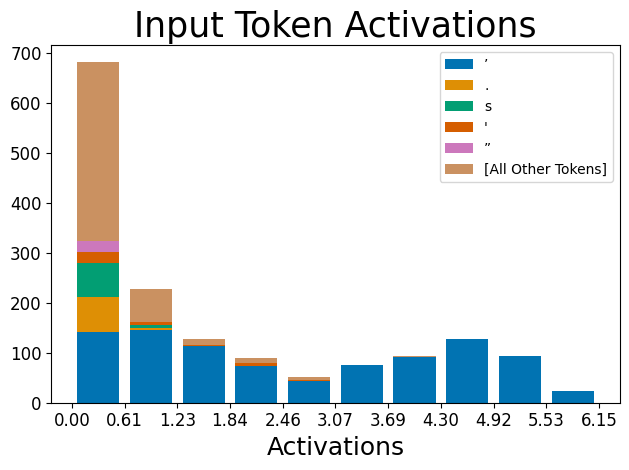
\includegraphics[width=.9\textwidth]{images/logan/apostrophe.png}
    \end{minipage}
    \hfill  % Optional: To make sure they are as far apart as possible.
    \begin{minipage}[b]{0.45\textwidth}
        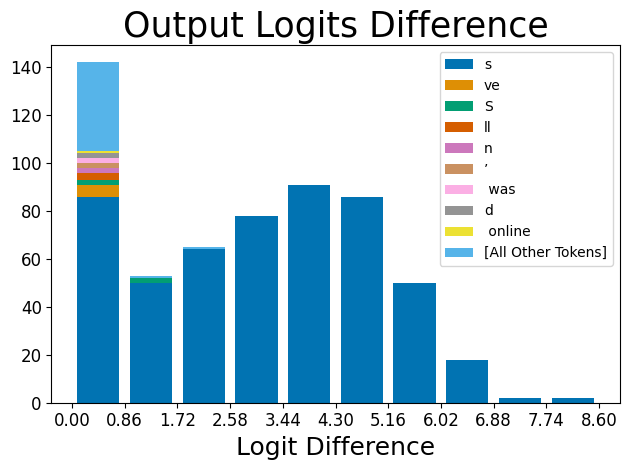
\includegraphics[width=.9\textwidth]{images/logan/apostrophe_effect_positive.png}
    \end{minipage}
    \caption{Histogram of token counts for dictionary feature 556. (Left) For all datapoints that activate dictionary feature 556, we show the count of each token in each activation range. The majority of activations are apostrophes, particularly for higher activations. Notably the lower activating tokens are conceptually similar to apostrophes, such as other punctuation. (Right) We show which token predictions are suppressed by ablating the feature, as measured by the difference in logits between the ablated and unablated model. We find that the token whose prediction decreases the most is the ``s'' token. Note that there are 12k logits negatively effected, but we set a threshold of 0.1 for visual clarity.}
    \label{fig:apostrophe}
\end{figure}

To better illustrate the monosemanticity of certain dictionary features, we plot the histogram of activations across token activations. This technique only works for dictionary features that activate for a small set of tokens. We find dictionary features that only activate on apostrophes (Figure \ref{fig:apostrophe}); periods; the token `` the''; and newline characters. The apostrophe feature in Figure \ref{fig:apostrophe} stands in contrast to the default basis for the residual stream, where the dimension that most represents an apostrophe is displayed in Figure \ref{fig:neuron_basis_apostrophe} in Appendix \ref{appendix:residual_stream_basis}; this dimension is polysemantic since it represents different information at different activation ranges. 


Although the dictionary feature discussed in the previous section activates only for apostrophes, it does not activate on \emph{all} apostrophes. This can be seen in Figures \ref{fig:ill_feature} and \ref{fig:dont_feature} in Appendix \ref{appendix:learned_features_examples}, showing two other apostrophe-activating dictionary features, but for different contexts (such as ``[I/We/They]'ll" and ``[don/won/wouldn]'t"). Details for how we searched and selected for dictionary features can be found in Appendix \ref{appendix:feature_search_details}.


\subsection{Output: Dictionary Features have Intuitive Effects on the Logits}
In addition to looking at which tokens activate the dictionary feature, we investigate how dictionary features affect the model's output predictions for the next token by ablating the feature from the residual stream\footnote{Specifically we use less-than-rank-one ablation, where we lower the activation vector in the direction of the feature only up to the point where the feature is no longer active.}. If our dictionary feature is interpretable, subtracting its value from the residual stream should have a logical effect on the predictions of the next token. We see in Figure \ref{fig:apostrophe} (Right) that the effect of removing the apostrophe feature mainly reduces the logit for the following ``s". This matches what one would expect from a dictionary feature that detects apostrophes and is used by the model to predict the ``s'' token that would appear immediately after the apostrophe in possessives and contractions like ``let's''. 

\subsection{Intermediate Features: Dictionary Features Allow Automatic Circuit Detection}
We can also understand dictionary features in relation to the upstream and downstream dictionary features: given a dictionary feature, which dictionary features in previous layers cause it to activate, and which dictionary features in later layers does it cause to activate?

To automatically detect the relevant dictionary features, we choose a target dictionary feature such as layer 5's feature for tokens in parentheses which predicts a closing parentheses (Figure \ref{fig:closing_parentheses_circuit}). For this target dictionary feature, we find its maximum activation $M$ across our dataset, then sample 20 contexts that cause the target feature to activate in the range $[M/2, M]$. For each dictionary feature in the previous layer, we rerun the model while ablating this feature and sort the previous-layer features by how much their ablation decreased the target feature. If desired, we can then recursively apply this technique to the dictionary features in the previous layer with a large impact. The results of this process form a causal tree, such as Figure \ref{fig:closing_parentheses_circuit}. 

Being the last layer, layer 5's role is to output directions that directly correspond to tokens in the unembedding matrix. In fact, when we unembed feature $5_{2027}$, the top-tokens are all closing parentheses variations. Intuitively, previous layers will detect all situations that precede closing parentheses, such as dates, acronyms, and phrases.
% , with examples shown in Table \ref{table:parentheses_examples}.

% \begin{table}[htb]
% \centering
% \begin{tabular}{@{}ll@{}}
% \toprule
% Description   & Example                                 \\ \midrule
% Acronyms      & The National Institute of Justice (NIJ) \\
% Dates         & NASA's Apollo 11 mission (1969)         \\
% Code          & If (x\%2==0):                           \\
% Induction     & You (1) wash your hands, then (2)       \\
% Abbreviations & Authors were HAL (Hoagy, Aidan, Logan)  \\ \bottomrule
% \end{tabular}
% \caption{Examples of various text that contains a closing parenthesis. A language model learning to predict the closing parenthesis would need to learn many different features, such as acronyms (specifically the end of them), dates (usually years), and asides (like this one). }
% \label{table:parentheses_examples}
% \end{table}

% \begin{landscape}
% \begin{figure}[p]
%     \centering
%     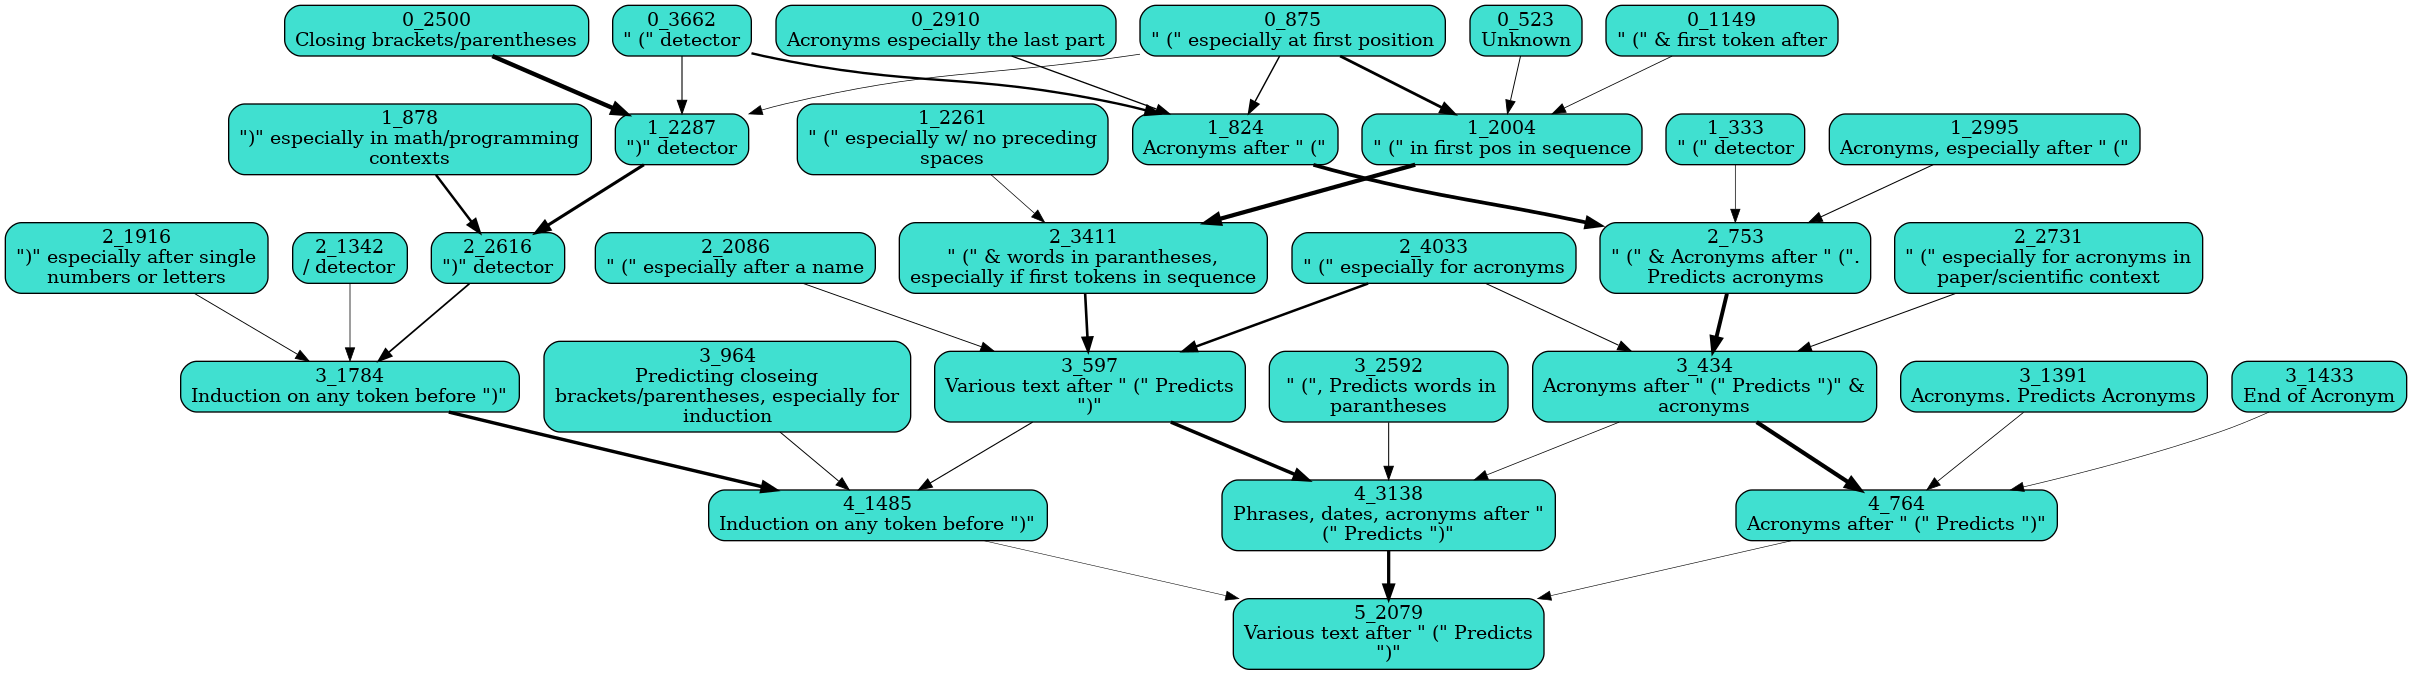
\includegraphics[scale=0.29]{images/logan/closing_parentheses_circuit.png}
%     \caption{Circuit for the closing parenthesis dictionary feature, with human interpretations of each feature shown. Edge thickness indicates the strength of the causal effect between dictionary features, as measured by ablations. Many dictionary features across layers correspond to similar real-world features and often point in similar directions in activation space, as measured by cosine similarity. For instance, dictionary features 0\_3662 and 1\_333 both detect ``(" and have a cosine similarity of 0.8, even though the diagram does not show them having a connection. This is an artifact of our automatic circuit-detection algorithm only back-chaining from the most relevant dictionary features found.}
%     \label{fig:closing_parentheses_circuit}
% \end{figure}

% \begin{landscape}
\begin{figure}[ht]
    \centering
    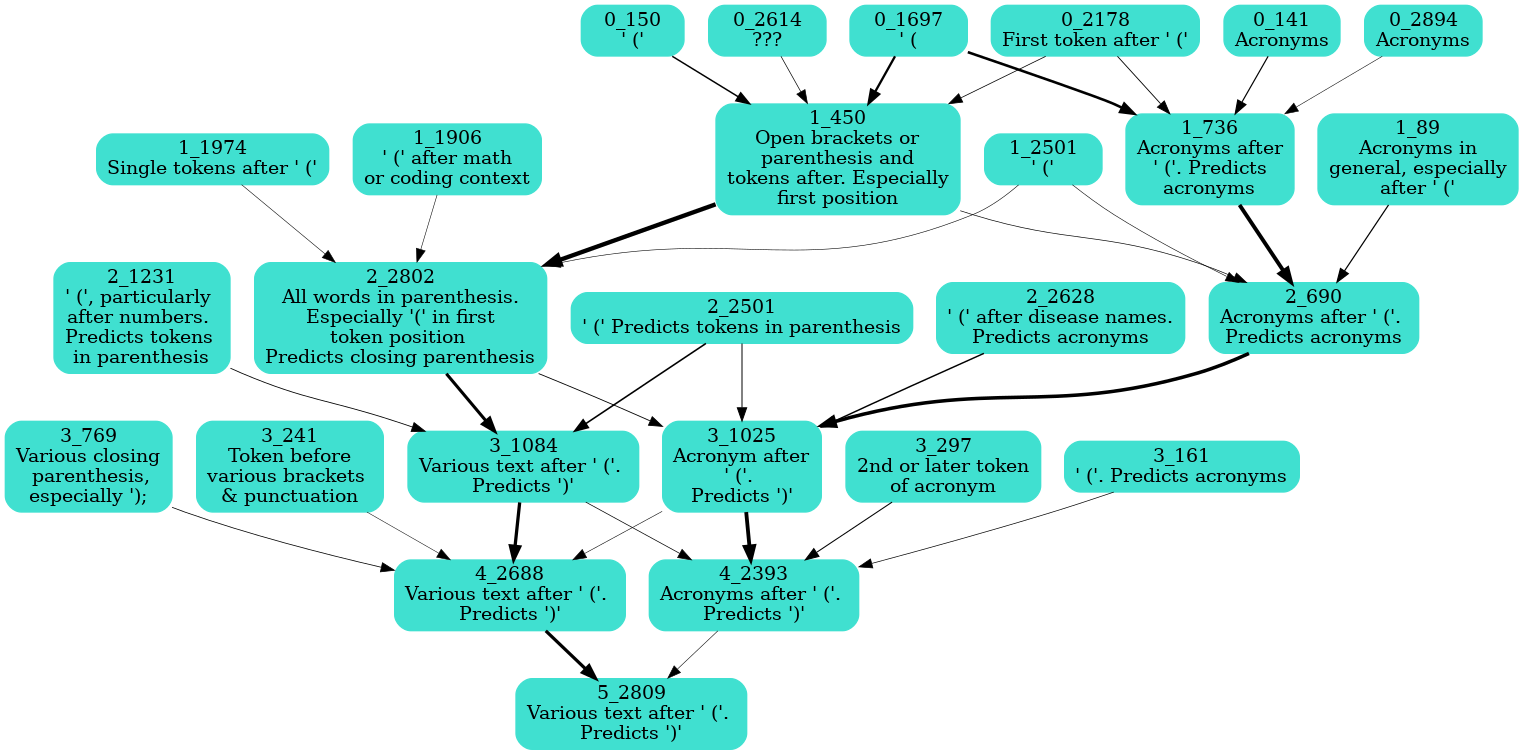
\includegraphics[width=\textwidth]{images/logan/close_paren_draft.png}
    \caption{Circuit for the closing parenthesis dictionary feature, with human interpretations of each feature shown. Edge thickness indicates the strength of the causal effect between dictionary features in successive residual stream layers, as measured by ablations. Many dictionary features across layers correspond to similar real-world features and often point in similar directions in activation space, as measured by cosine similarity.}
    \label{fig:closing_parentheses_circuit}
\end{figure}

% \end{landscape}
